%=============================================================================
% Methodology
% Copyright (c) 2018. Lester James V. Miranda
%
% This file is part of thesis-manuscript.
%
% thesis-mansucript is free software: you can redistribute it and/or modify
% it under the terms of the GNU General Public License as published by
% the Free Software Foundation, either version 3 of the License, or
% (at your option) any later version.
%
% thesis-manuscript is distributed in the hope that it will be useful,
% but WITHOUT ANY WARRANTY; without even the implied warranty of
% MERCHANTABILITY or FITNESS FOR A PARTICULAR PURPOSE.  See the
% GNU General Public License for more details.
%
% You should have received a copy of the GNU General Public License
% along with thesis-manuscript.  If not, see <http://www.gnu.org/licenses/>.
%
% Created by: Lester James V. Miranda <ljvmiranda@gmail.com>
%=============================================================================

\chapter{Proposed Method}
\label{Methodology}

% Write overview here, talk about the training and test phases.

\par The entire protein function prediction model consists of two stages: (1) a
\textit{feature extraction} stage that extracts new representations from
raw data, and a \textit{multi-label classification} stage that assigns each
protein sample to its respective set of functions. During training, the
model learns the parameters $\theta$ and $W$ for the two stages separately.
At inference, matrix operations are only applied to transform the input data
and predict protein functions. An illustration for the training and test phases
can be found at Figure \ref{schema:training_testing}. \footnote[2]{The subscripts
$tr$ and $ts$ refer to the training and test data respectively.} The proposed
autoencoder network resides in the first stage.

\par This chapter will discuss in detail the algorithm in Section
\ref{FeatureExtraction}, and the multi-label classifier in Section
\ref{MultiLabelClassification}. Lastly, an overview of the
datasets and experimental environment will be described in Sections
\ref{Datasets} and \ref{ExperimentalEnvironment} respectively.


\begin{figure}[h]
    \centering
    \begin{subfigure}[b]{0.8\textwidth}
        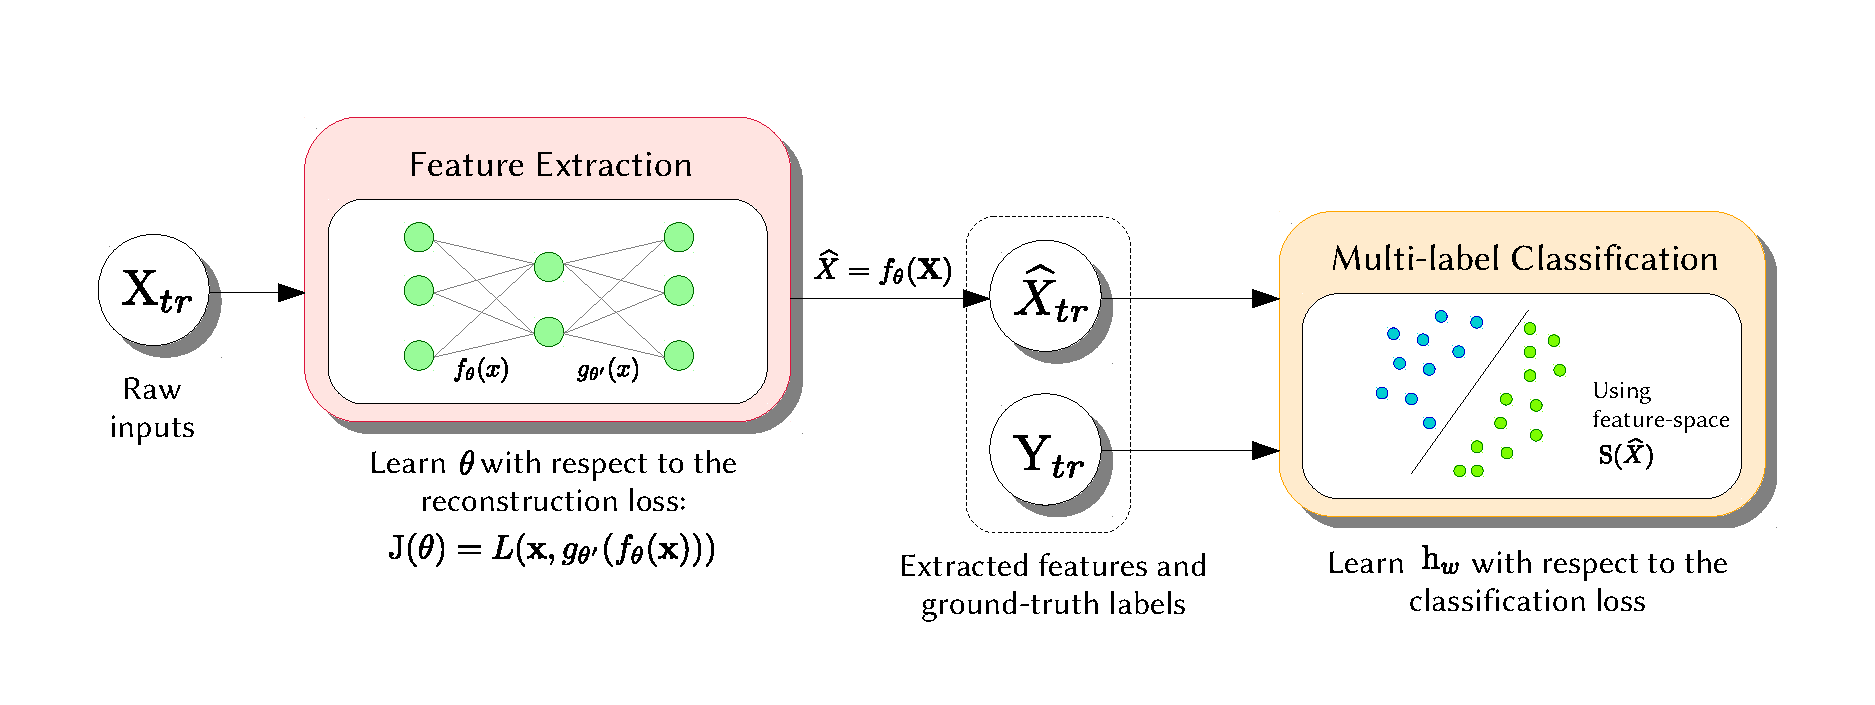
\includegraphics[width=\textwidth]{ch03/schema_training}
        \caption{Training phase}
        \label{schema:training}
    \end{subfigure}
    ~ %add desired spacing between images, e. g. ~, \quad, \qquad, \hfill etc. 
      %(or a blank line to force the subfigure onto a new line)
    \begin{subfigure}[b]{0.9\textwidth}
        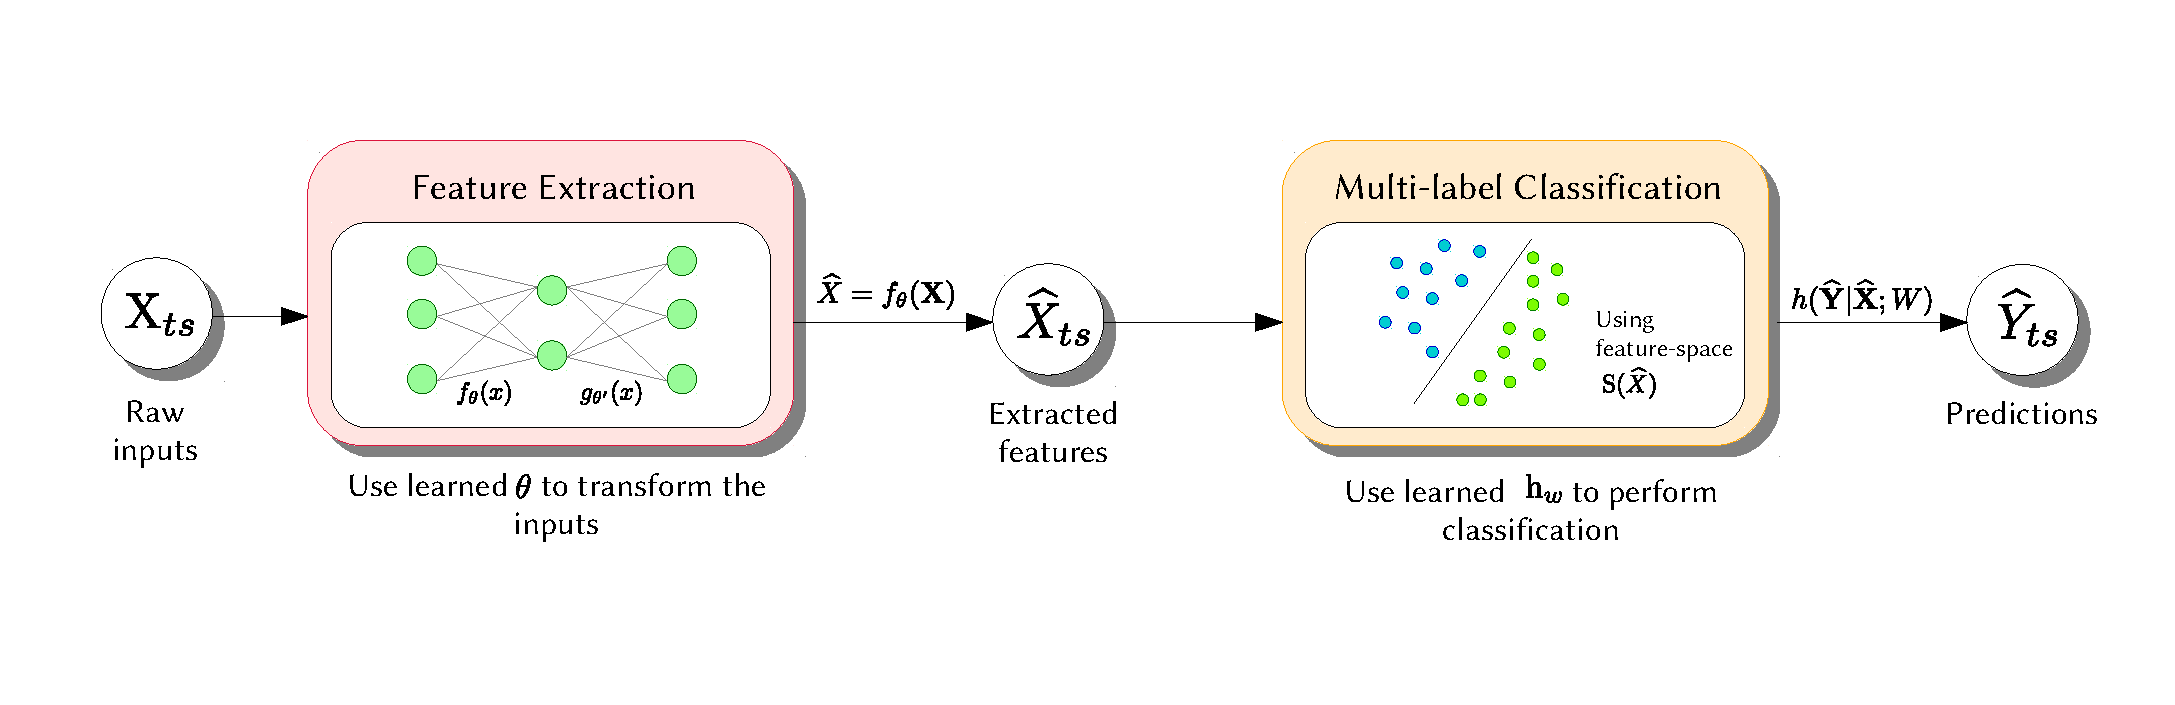
\includegraphics[width=\textwidth]{ch03/schema_testing}
        \caption{Testing phase}
        \label{schema:testing}
    \end{subfigure}
    \caption{Train and test phases for the protein function prediction model}
    \label{schema:training_testing}
\end{figure}

\section{Feature Extraction}
\label{FeatureExtraction}

\par This stage consists of the proposed autoencoder network for selective
feature extraction. Selecting relevant features is achieved through mutual
competition. All of this happens at the training phase and is accomplished
by performing the following tasks:

\begin{itemize}
    \item A winner-take-all operation selects the top k\% neurons or 
        \textit{winners} depending on their activation value; and
    \item A sparse operation redistributes the activation of the non-k\%
        neurons or \textit{losers} to the winners. This results to a sparse
        layer highlighting the winning or relevant neurons.
\end{itemize}

\noindent  Figure \ref{schema:proposed} illustrates the proposed network.
At testing, the two operations are simply turned-off. The network uses the
learned weights from training to determine and transform the relevant features
from the input test data.

\par From this design, three hyperparameters can be adjusted:

\begin{itemize}
    \item The encoding layer size, $e$, that controls how many features
        should be extracted from the raw data. (If $e>d$ then the network is
        overcomplete, otherwise it is undercomplete).
    \item The percent sparsity $k\%$ that determines the number of winners $w$
        retained during the winner-take-all operation.
    \item The competition parameter $\alpha$ that adjusts the amount of activation
        from the losers to be distributed to the winners.
\end{itemize}

\begin{figure}[h]
    \centering
    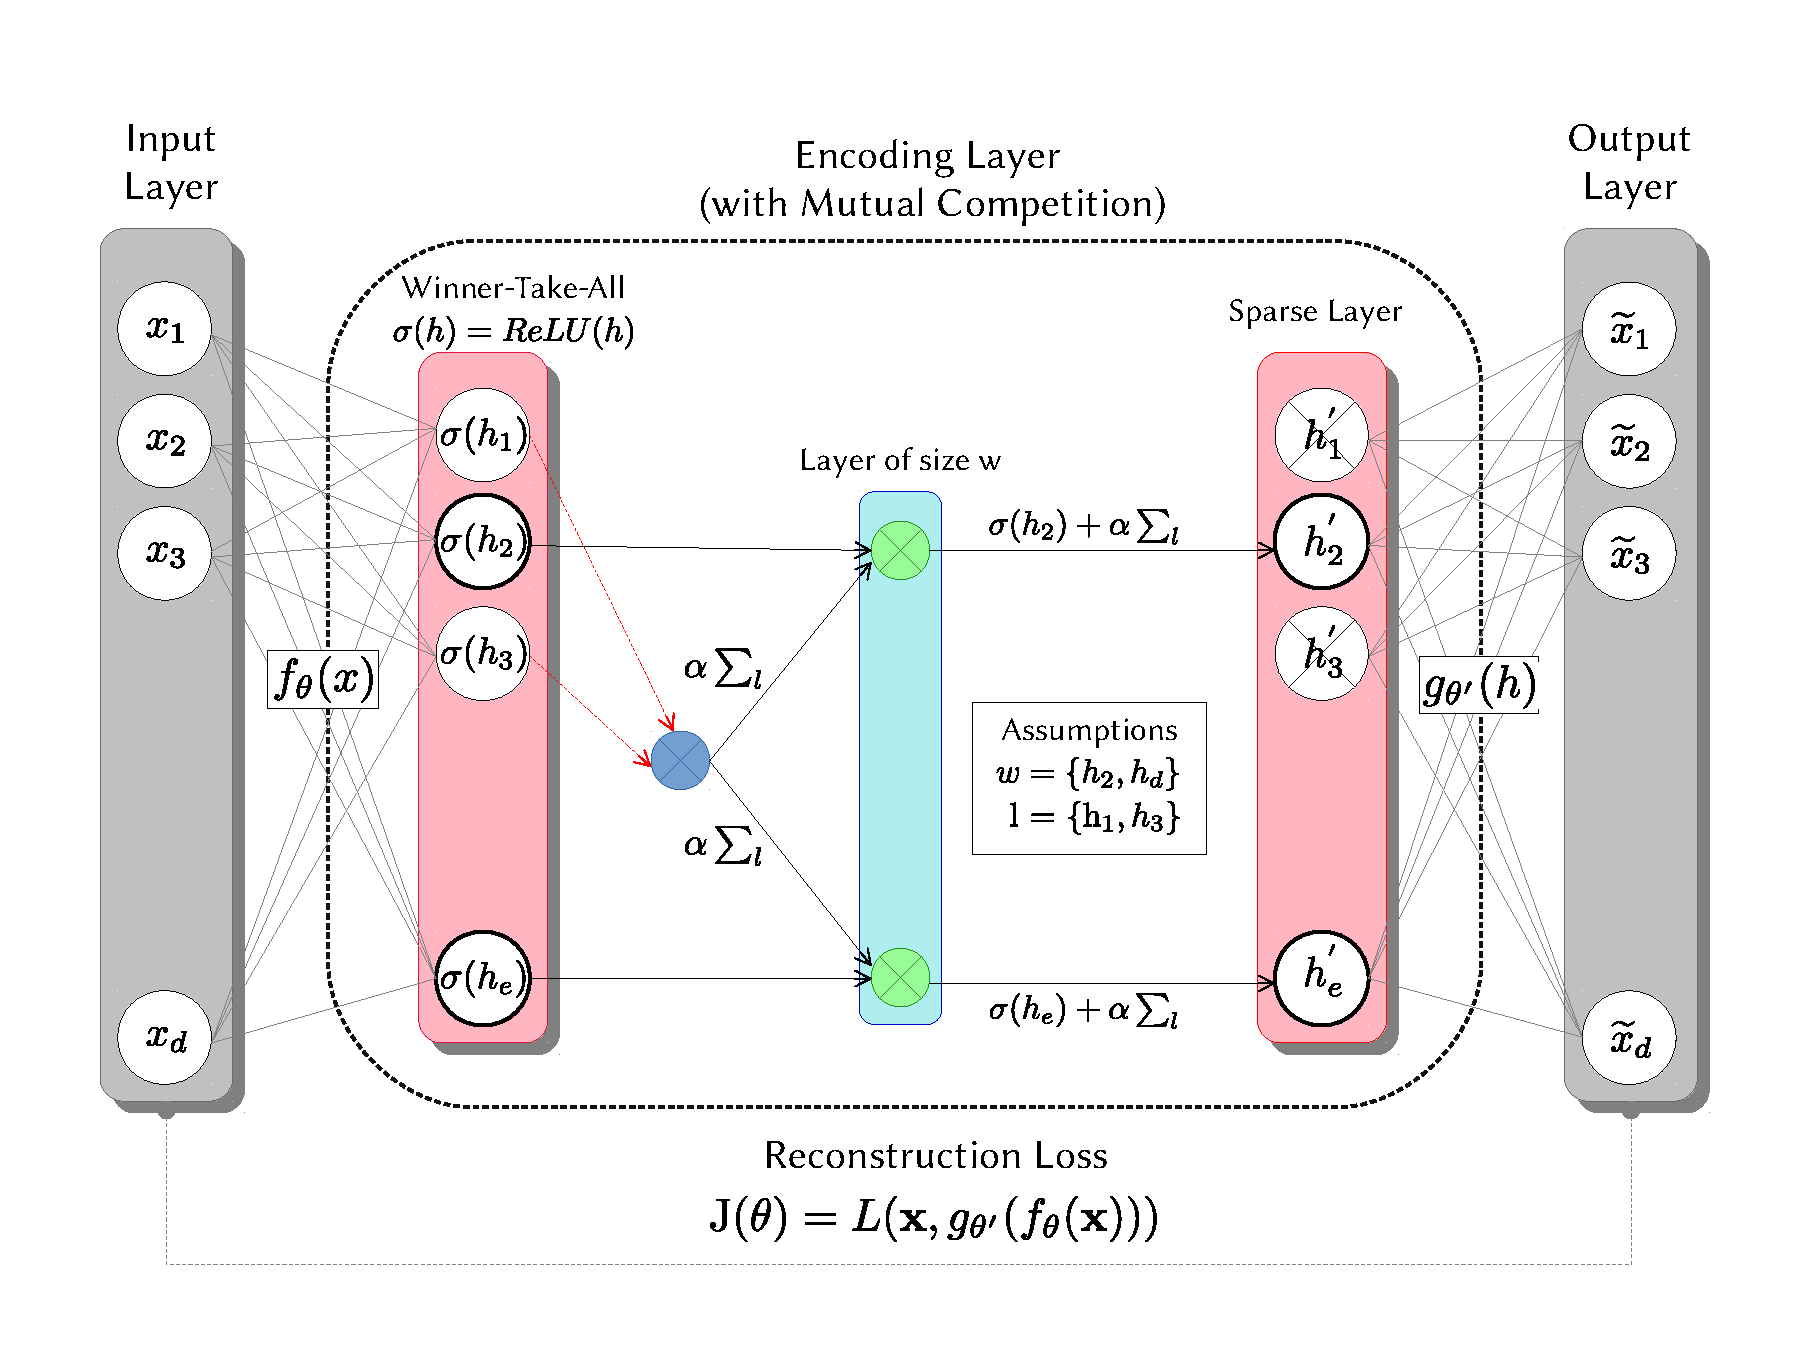
\includegraphics[width=0.75\textwidth]{ch03/schema_proposed}
    \caption[Proposed autoencoder network with mutual competition]
    {The proposed autoencoder network with mutual competition}
    \label{schema:proposed}
\end{figure}

\par Algorithm \ref{algo:training} gives an overview of the training procedure
for the proposed method. The autoencoder starts off by initializing the weight
parameters randomly from a normal distribution. Then, for a set number of
epochs, a feedforward step with ReLU activation maps the inputs $\mathbf{x}$
to the encoding dimension $\mathbf{h}$ of size $e$. A winner-take-all
operation creates a dictionary of all $k$ winners and losers to set-up the
sparse layer. The layer contains the winners with their updated
activations from the losers as controlled by $\alpha$. Afterwards, the
decoder function will attempt to reconstruct the input from the sparse layer.
This finally initiates the backpropagation routine to update the parameters
$\theta$. At the end of training, the model parameters are returned.

%=============================================================================
% algo-training.tex
% Copyright (c) 2018. Lester James V. Miranda
%
% This file is part of thesis-manuscript.
%
% thesis-mansucript is free software: you can redistribute it and/or modify
% it under the terms of the GNU General Public License as published by
% the Free Software Foundation, either version 3 of the License, or
% (at your option) any later version.
%
% thesis-manuscript is distributed in the hope that it will be useful,
% but WITHOUT ANY WARRANTY; without even the implied warranty of
% MERCHANTABILITY or FITNESS FOR A PARTICULAR PURPOSE.  See the
% GNU General Public License for more details.
%
% You should have received a copy of the GNU General Public License
% along with thesis-manuscript.  If not, see <http://www.gnu.org/licenses/>.
%
% Created by: Lester James V. Miranda <ljvmiranda@gmail.com>
%=============================================================================

\begin{algorithm}
\caption{Training the proposed autoencoder network}
\label{algo:training}
\begin{algorithmic}[1]

\INPUT Training examples $\mathbf{X}$, competition parameter $\alpha$, percent sparsity $k\%$
\OUTPUT Model weights $\theta$, extracted features $\mathbf{\widehat{X}}$

\item[]
\Procedure{Initialization}{}
    \State $\theta_{i}^{(0)} \gets \mathcal{N}(\mu,\,\sigma^{2})$
    \Comment{Initialize weights}
    \State $\theta_{0}^{(0)} \gets \mathcal{N}(\mu,\,\sigma^{2})$
    \Comment{Initialize biases}
\EndProcedure

\item[]
\Procedure{Training}{}
    \For{\textit{NumEpochs}}
        \State Feedforward propagation: $\mathbf{h} \gets f_{\theta}(\mathbf{X}) =
        \sigma(\theta\mathbf{X}^{T}+\theta_{0})$
        \Comment Until last encoding layer
        \State $D \gets$ \Call{WinnerTakeAll}{$\mathbf{h}$, $k$}
        \Comment Store winners and losers in a dictionary
        \State $\mathbf{h'} \gets$ \Call{Sparse}{$D$, $\alpha$}
        \State Compute output: $\mathbf{\widetilde{X}} \gets 
        g_{\theta'}(\mathbf{h'}) = \sigma(\theta'\mathbf{h'}^{T}+\theta_{0})$
        \Comment Tied weights, $\theta'=\theta^{T}$
        \State Compute reconstruction error $\mathbf{J}_{\theta}$
        \State \Call{Backpropagation}{$\mathbf{J}_{\theta}$}
        \Comment Only for winning neurons
    \EndFor
    \State \Return $\theta$ 
\EndProcedure

\item[]
\Procedure{Transform}{$\mathbf{X}$}
    \State
    $\mathbf{\widehat{X}}=f_{\theta}(\mathbf{X})=\sigma(\theta\mathbf{X}^{T} +
    \theta_{0})$
    \State \Return $\mathbf{\widehat{X}}$
\EndProcedure

\end{algorithmic}
\end{algorithm}


\par When performing a feature transform, we use the encoder function
$f_{\theta}$ to map the input into its new representation. The extracted
features $\mathbf{\widehat{X}}$ has a size $e$ as determined from training.
The winner-take-all and sparse operations are turned-off during this process.
Further details on these operations will be discussed in the proceeding
sections.

\subsection{Winner-take-all operation}

\par The winner-take-all operation retains the top $k$\% neurons
in a given layer based on its activation. Thus, after the feedforward phase,
instead of directly reconstructing the encoded data, a percentage of
neurons in the last encoding layer are kept by the network. In this manner, a
lifetime sparsity is enforced and the rest of the non-$k$\% neurons
(or ``losers'') are set to $0$ by the sparse operation later.

\par During the backpropagation phase, the error is only passed through
the non-zero neurons in the hidden layers. When performing a feature transform
, this operation is ignored. Since the weights were trained with
respect to the ``winners,'' it enables the model to distinguish the
corresponding neurons. Algorithm \ref{algo:wta} describes this procedure.

%=============================================================================
% algo_wta.tex
% Copyright (c) 2018. Lester James V. Miranda
%
% This file is part of thesis-manuscript.
%
% thesis-mansucript is free software: you can redistribute it and/or modify
% it under the terms of the GNU General Public License as published by
% the Free Software Foundation, either version 3 of the License, or
% (at your option) any later version.
%
% thesis-manuscript is distributed in the hope that it will be useful,
% but WITHOUT ANY WARRANTY; without even the implied warranty of
% MERCHANTABILITY or FITNESS FOR A PARTICULAR PURPOSE.  See the
% GNU General Public License for more details.
%
% You should have received a copy of the GNU General Public License
% along with thesis-manuscript.  If not, see <http://www.gnu.org/licenses/>.
%
% Created by: Lester James V. Miranda <ljvmiranda@gmail.com>
%=============================================================================


\begin{algorithm}
    \caption{Winner-Take-All operation}
    \label{algo:wta}
    \begin{algorithmic}[1]
    
    \INPUT Output of last encoding layer $\mathbf{h}$, percent sparsity $k\%$
    \OUTPUT Dictionary of winners and losers, $D = \{\}$

    \item[]
    \State \textit{LayerSize} $\gets$ length($\mathbf{h}$)
    \Comment Get number of units in the layer
    \State \textit{NeuronsToKeep} $\gets k\% * \text{\textit{LayerSize}}$
    \State $D[\text{Winners}] \gets$ first \textit{NeuronsToKeep} in \Call{SortAscendingOrder}{$\mathbf{h}$}
    \State $D[\text{Losers}] \gets$ remaining neurons in \Call{SortAscendingOrder}{$\mathbf{h}$}
    \State \Return $D$
    \end{algorithmic}
\end{algorithm}


\subsection{Sparse operation}

\par The sparse operation allows the winner neurons to ``soak-up'' the
activation of the loser neurons. This is done via an adder controlled by
a hyperparameter $\alpha$. Boosting the energy of the winning neurons can
affect the backpropagation path so that weights are optimized in their favor.
This assumes that the winners, due to their high activation, are the
relevant features representing the input data. Algorithm \ref{algo:sparse}
describes this operation.

%=============================================================================
% algo_sparse.tex
% Copyright (c) 2018. Lester James V. Miranda
%
% This file is part of thesis-manuscript.
%
% thesis-mansucript is free software: you can redistribute it and/or modify
% it under the terms of the GNU General Public License as published by
% the Free Software Foundation, either version 3 of the License, or
% (at your option) any later version.
%
% thesis-manuscript is distributed in the hope that it will be useful,
% but WITHOUT ANY WARRANTY; without even the implied warranty of
% MERCHANTABILITY or FITNESS FOR A PARTICULAR PURPOSE.  See the
% GNU General Public License for more details.
%
% You should have received a copy of the GNU General Public License
% along with thesis-manuscript.  If not, see <http://www.gnu.org/licenses/>.
%
% Created by: Lester James V. Miranda <ljvmiranda@gmail.com>
%=============================================================================

\begin{algorithm}
    \caption{Sparse operation}
    \label{algo:sparse}
    \begin{algorithmic}[1]
    
    \INPUT Dictionary of winners and losers $D = \{\}$, competition parameter $\alpha$
    \OUTPUT Updated activation of winners and losers $\mathbf{h}'$

    \item[]
    \State \textit{ToAllocate} $\gets$ \Call{Sum}{$D[Losers]$}
    \Comment Sum all activations of loser neurons
    \State $\mathbf{a}_{w} \gets$ $D[Winners]$ + $\alpha$ \textit{ToAllocate}
    \Comment Update activation of winners, $\mathbf{a}_{w}$
    \State $\mathbf{a}_{l} \gets 0$ 
    \Comment Set activation of losers to $0$.
    \State \textbf{return} $\mathbf{h}' = \{\mathbf{a}_{w}$, $\mathbf{a}_{l}\}$
    \end{algorithmic}
\end{algorithm}


\section{Multi-label Classification}
\label{MultiLabelClassification}

\par Once extracted, the new features will be sent to a multi-label classifier for
inference. We train the classifier $h$, and learn its parameters $W$. In this
research, $h$ comes in the form of a binary-relevance support-vector machine
(BR-SVM), and is trained with respect to the SVM squared hinge loss (L2-SVM): 

\begin{equation}
J_i = \sum_{\widehat{\mathbf{y}}_i \neq \mathbf{y}_i}\max(0, W_{\widehat{\mathbf{y}}}^{T} \mathbf{x}_{i}^{'} - W_{\mathbf{y}_i}^{T}\mathbf{x}_{i}^{'} + \Delta)^{2}
\end{equation}

\par During SVM training, two library implementations were used: LIBSVM and
LIBLINEAR for the gaussian and linear kernels respectively
(\cite{chang2011libsvm, fan2008liblinear}). However, given large datasets, the
SVM algorithm can reach a time-complexity between $\mathcal{O}(n^{2})$ and
$\mathcal{O}(n^{3})$ (\cite{bottou2006support}). If we account for the
additional complexity of binary-relevance for each label, then the overall
training time will be longer. To resolve this problem, distributed training was
implemented.

\par Figure \ref{schema:multiprocessing} outlines this procedure. The training
dataset was partitioned into $N$ batches, and was distributed to $N$ jobs. The
protein samples for each partition were chosen randomly without replacement and
is assigned into its own thread. Because there are less number of samples for
each SVM classifier, training becomes much faster. Finally, the validation score
is obtained by averaging the results of all partitions for each label
$\lambda$. This results to a trained classifier $h(\mathbf{Y} \given
\mathbf{\widehat{X}}; \mathbf{W})$ for inferring the test data.

\begin{figure}[t]
    \centering
    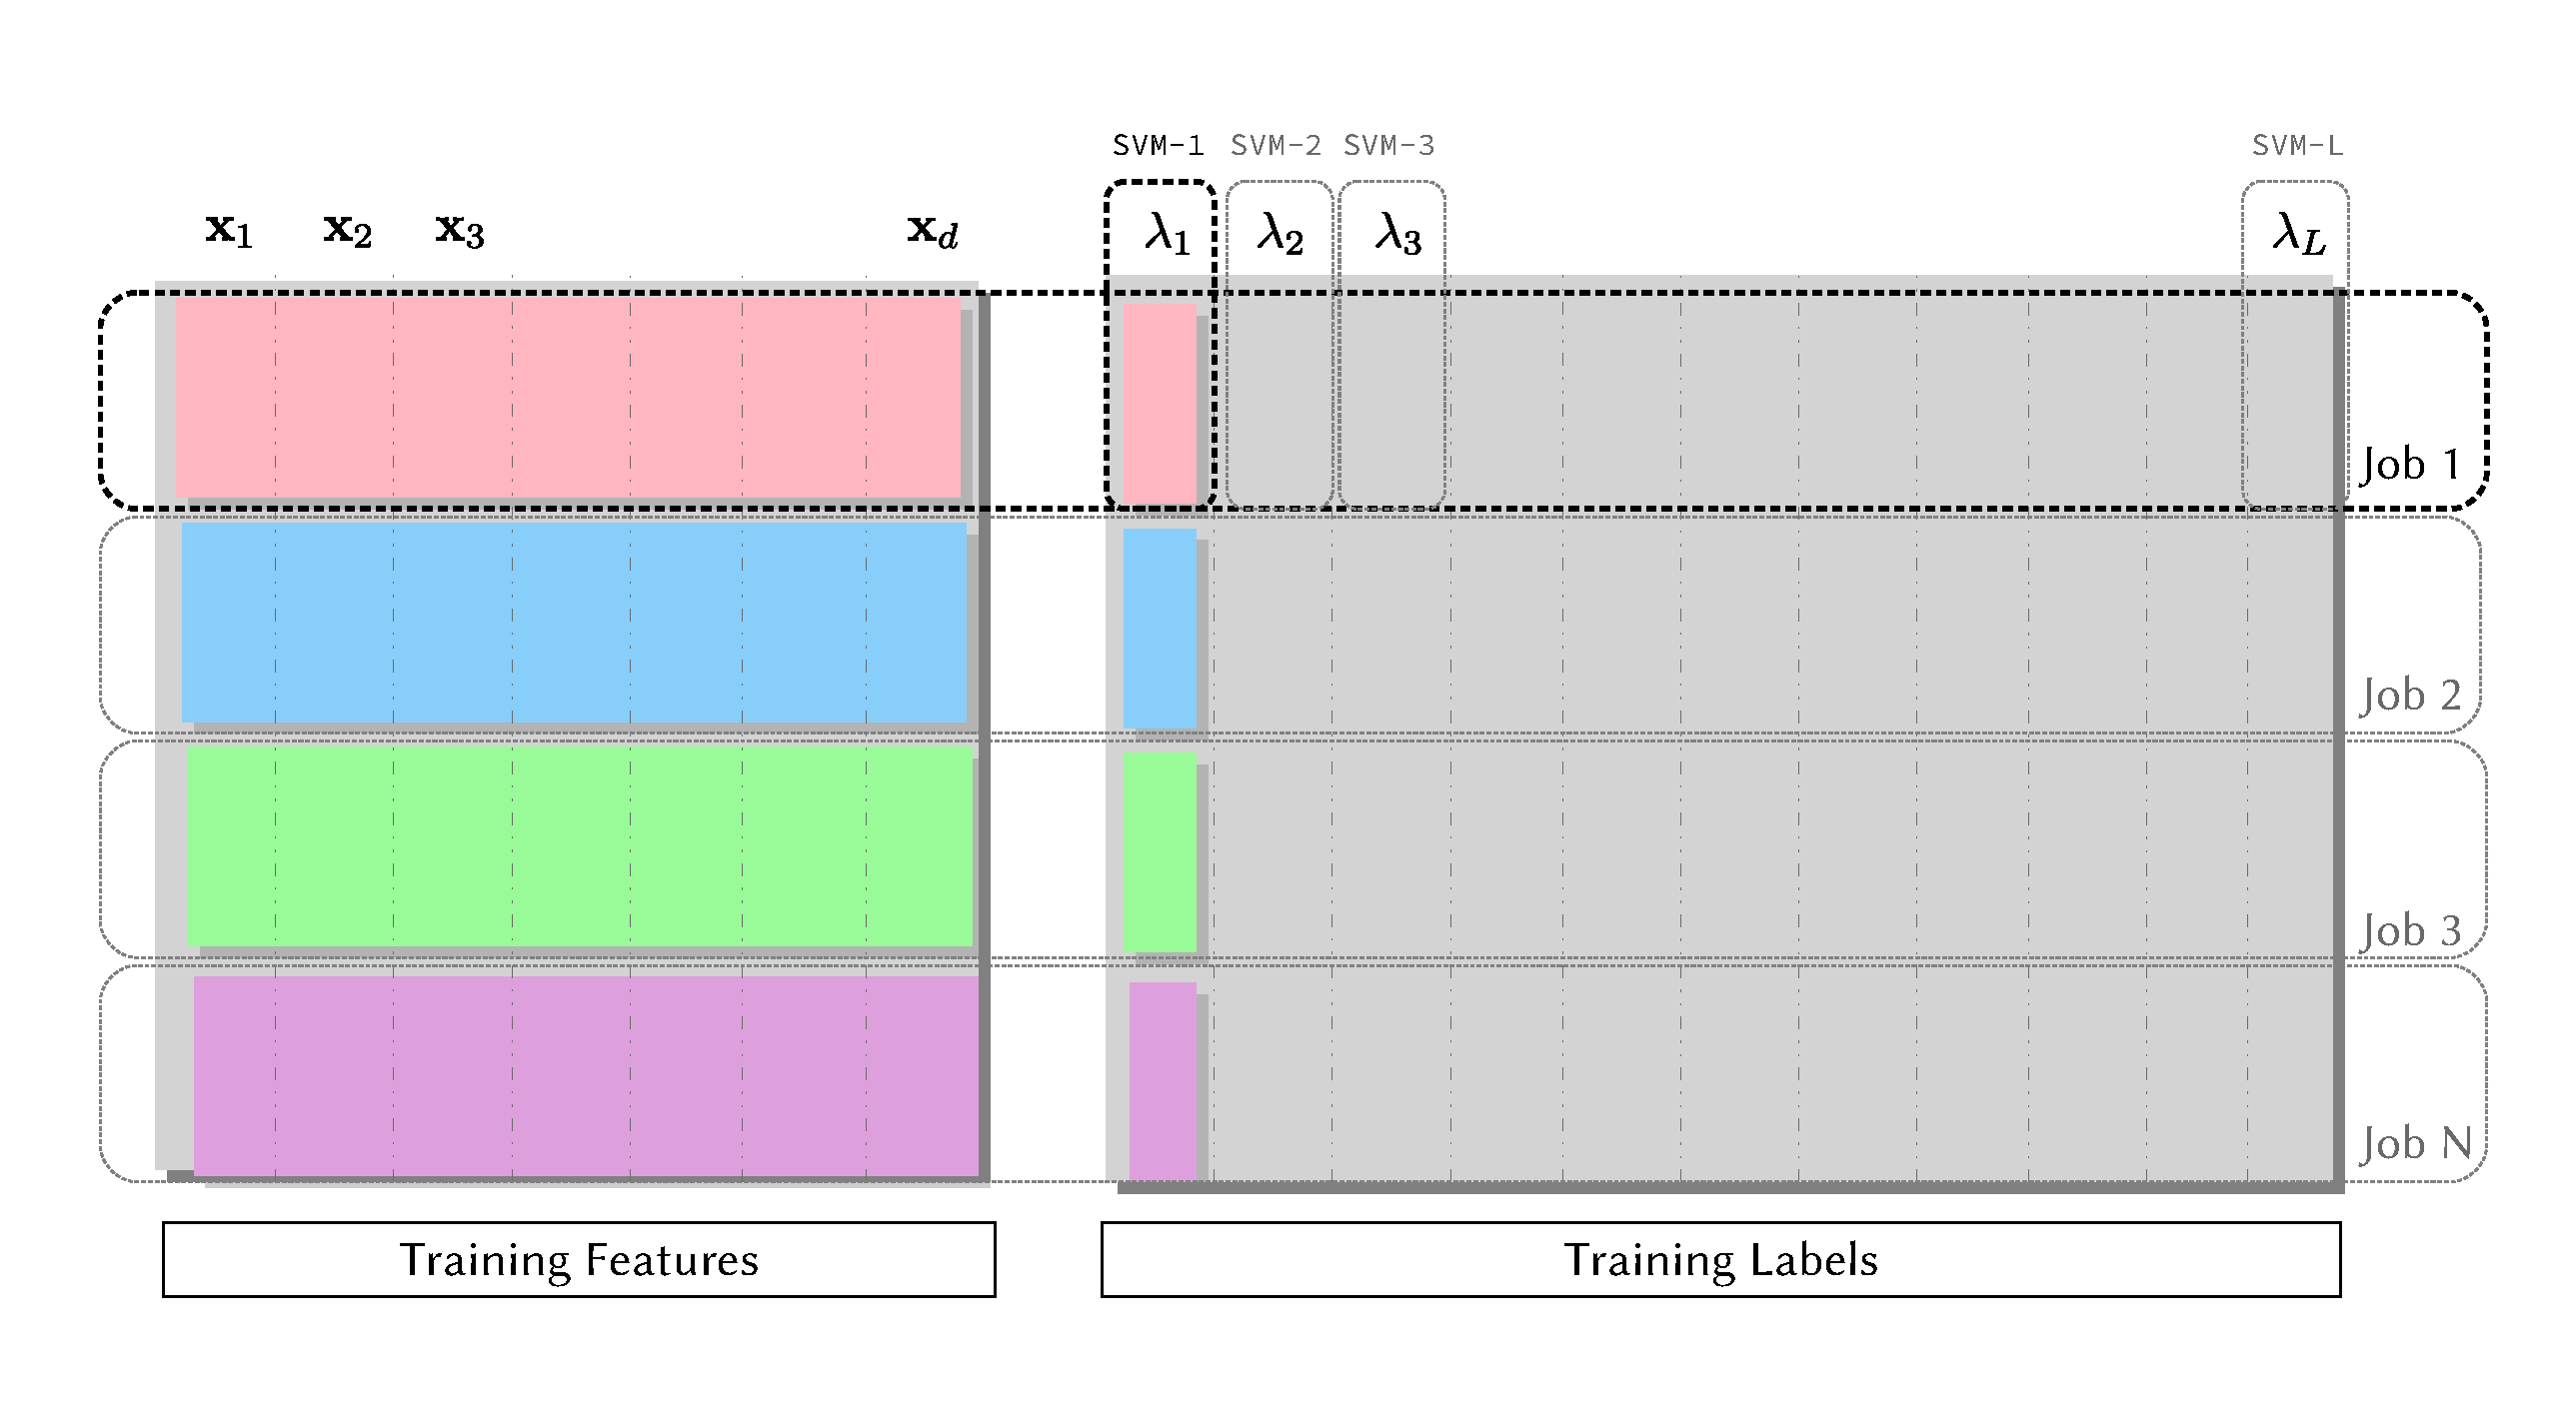
\includegraphics[width=0.75\textwidth]{ch03/schema_multiprocessing}
    \caption[Distributed approach in training multiple BR-SVMs]
    {Distributed approach in training multiple BR-SVMs. The training dataset
    was partitioned into $N$ jobs where each is assigned into a thread.}
    \label{schema:multiprocessing}
\end{figure}

\subsection{Evaluation Metrics}

To evaluate the performance of the prediction model, we will use the following
metrics\footnote[2]{\textit{tp}: true positive, \textit{fp}:
false positive, \textit{tn}: true negative, \textit{fn}: false negative}:

\begin{align}
    \text{Hamming Loss (H)} &= \dfrac{1}{N \cdot L} \sum_{i=1}^{N} \sum_{j=1}^{L}
    \text{XOR}(y_{ij}, \widehat{y}_{ij}) \\
    \text{Precision (P)} &=
    \dfrac{1}{N}\sum_{i=1}^{N}\dfrac{|\mathbf{\widehat{y}}_{i} \cap
    \mathbf{y}_{i}|}{|\mathbf{\widehat{y}_{i}}|} = \dfrac{tp}{tp + fp} \\
    \text{Recall (R)} &=
    \dfrac{1}{N}\sum_{i=1}^{N}\dfrac{|\mathbf{\widehat{y}}_{i} \cup
    \mathbf{y}_{i}|}{|\mathbf{\widehat{y}_{i}}|} = \dfrac{tp}{tp + fn} \\
    \text{F-score (F)} &=
    \dfrac{1}{N}\sum_{i=1}^{N} \dfrac{2 | \mathbf{\widehat{y}}_{i} \cup
        \mathbf{y}_{i}|}{|\mathbf{\widehat{y}}_{i} | + |\mathbf{y}_{i}|} =
        \dfrac{2 (\text{P} \cdot \text{R})}{\text{P} +
        \text{R}}
\end{align}

\par We will also compute for a fifth metric, the Area Under the ROC Curve
(AUROC), to serve as proxy for accuracy. Together with the Hamming loss and
F-score, the model will be evaluated and compared to other works. Lastly,
the Precision-Recall score will determine the quality of our model in terms of
sensitivity and specificity.

\par In addition, the AUROC, F-score, and Precision-Recall will be averaged
in three ways: micro (\textit{mi}), macro (\textit{ma}), and by-samples
(\textit{sa}). As an illustration, given $L$ labels and $N$ samples, a
micro-averaged precision ($P_{mi}$) is computed using the true-positives and
false-positives of each label and averaged:

\[
    P_{mi} = \dfrac{\sum_{i=1}^{L} tp_{i}}{\sum_{i=1}^{L} tp_{i} +
    \sum_{i=1}^{L} fp_{i}}
\]

\noindent In macro-averaging, the precision for each label is computed and
averaged. Because this metric is weighted, they are affected by
the number of true instances for each label $l$. This weighing scheme
offsets class imbalance:

\[
    P_{ma} = \dfrac{1}{L} \sum_{i=1}^{L} w_{i} P_{i}
\]

\noindent Lastly, in samples averaging, the metrics are computed for each
instance $m$ and averaged by the number of samples:

\[
    P_{samples} = \dfrac{1}{M}\sum_{i=1}^{M} P_{i}
\]

\noindent Averaging in this manner creates a stricter set of metrics
consistent with other works in literature (\cite{madjarov2012extensive,
gibaja2015tutorial, herrera2016multilabel, tsoumakas2017data}).

\section{Datasets}
\label{Datasets}

\par Two benchmark datasets will be studied in this work. First is the
\textbf{yeast} dataset that contains micro-array expression data and
phylogenetic profiles of 1500 genes in \textit{Saccharomyoes cerevisiae} or
baker's yeast (\cite{elisseeff2001kernel}). Second is the \textbf{genbase}
dataset containing protein sites and motif data of the ten most important
protein families\footnote[2]{The protein families are described in terms of
their Prosite documenation ID (\cite{diplaris2005protein,
bairoch1991prosite,hatzidamianos2003genminer}): PDOC00064 (oxydoreductases),
PDOC00154 (isomerases), PDOC00224 (cytokines and growth factors), PDOC00343
(structural proteins), PDOC00561 (receptors), PDOC00662 (DNA or RNA associated
proteins), PDOC00670 (transferases), PDOC00791 (protein secretion and
chaperones), and PDOC50007 (hydrolases).} (\cite{diplaris2005protein}). Table
\ref{setup:datasets} provides their description.

\par Recall that labelsets are represented as a binary matrix $\mathbf{Y} \in
\{0,1\}^{M \times N} $ where $\lambda_{mn} = 1$ if protein sample $m$ has
function $n$ and $0$ otherwise. Here, cardinality represents the average
number of active labels ($\lambda_{mn}=1$) per instance. Thus, a $4.237$ value
in yeast indicates that each sample is associated with slightly more than $4$
labels on average. On the other hand, density describes labelset sparsity. A
value of $0.0460$ in genbase means that around $4.6\%$ of labels are active.

\par To illustrate the multi-label aspect of the two datasets, Figure
\ref{graph:cooccurence} shows a co-occurence plot. Each arc in the circle
corresponds to a protein function in the dataset. The width of the arc
represents its frequency. Each chord connecting any two arcs depicts their
simultaneous presence in a protein sample.


\begin{table}[t]
    \centering
    \caption{Dataset description}
    \label{setup:datasets}
    \begin{tabular}{@{}rrrrrr@{}}
        \toprule
        Dataset & Instances & Features & Labels & Cardinality & Density    \\ \midrule
        yeast   & $2417$      & $103$      & $14$     & $4.237$       & $0.3030$     \\
        genbase & $662$       & $1186$     & $27$     & $1.252$       & $0.0460$     \\ \bottomrule
    \end{tabular}
\end{table}


\begin{figure}[t]
    \centering
    \begin{subfigure}[b]{0.49\textwidth}
        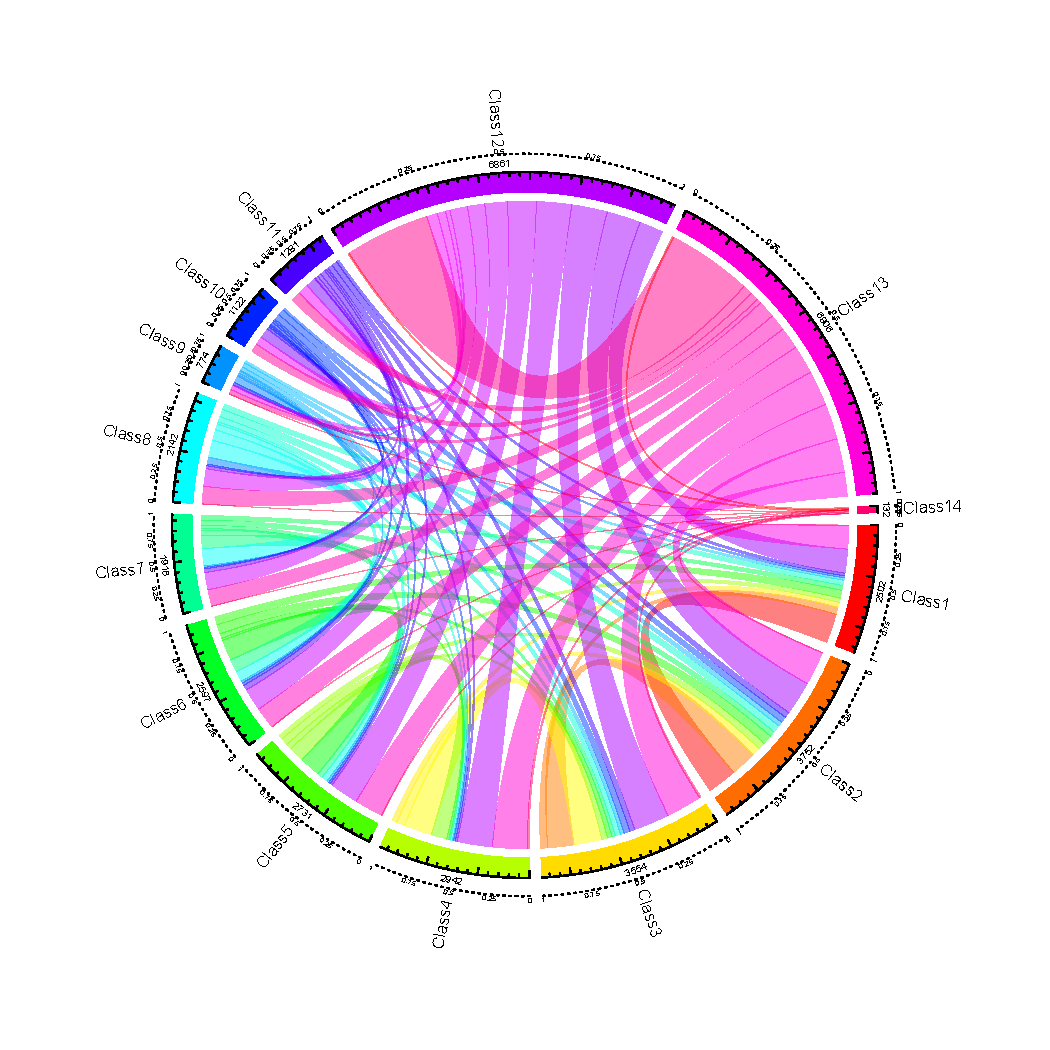
\includegraphics[width=\textwidth]{ch03/graph_yeast}
        \caption{Yeast}
        \label{graph:yeast}
    \end{subfigure}
    ~ %add desired spacing between images, e. g. ~, \quad, \qquad, \hfill etc. 
      %(or a blank line to force the subfigure onto a new line)
    \begin{subfigure}[b]{0.49\textwidth}
        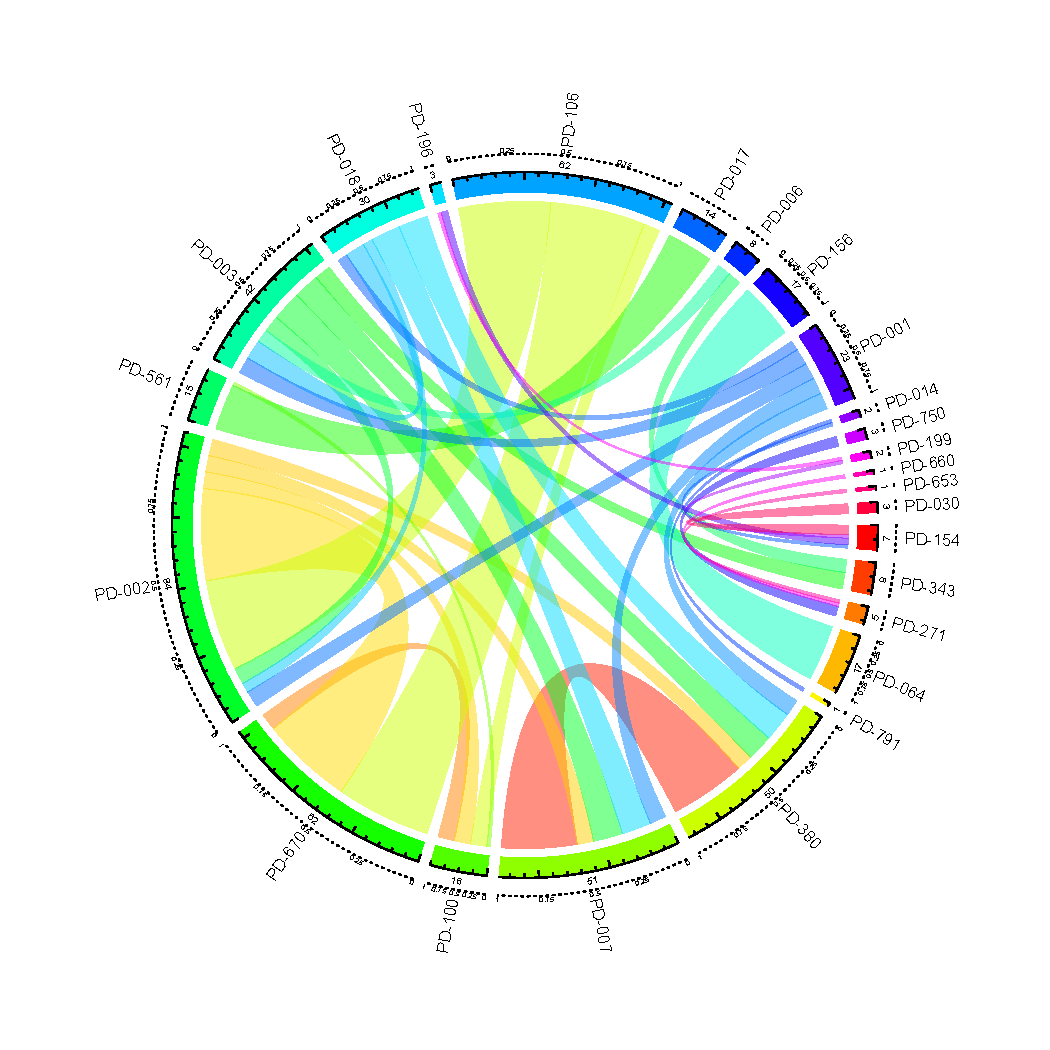
\includegraphics[width=\textwidth]{ch03/graph_genbase}
        \caption{Genbase}
        \label{graph:genbase}
    \end{subfigure}
    \caption[Co-occurence plot for the yeast and genbase datasets]
    {Co-occurence plot for the yeast and genbase datasets. Each arc corresponds
    to a particular class where each chord indicates their simultaneous
    presence on a given protein sample}
    \label{graph:cooccurence}
\end{figure}

\section{Experimental Environment}
\label{ExperimentalEnvironment}

Table \ref{setup:environment} describes the environment used for the
experiments. The GPU was used to train the neural network, and the CPU for
training the classifier. Only ten (10) out of the forty cores were used
simultaneously during the experiments. The source code can be obtained from
\url{https://github.com/ljvmiranda921/PFPredict}. It uses the Tensorflow
library to construct the proposed network and runs on both Python 2.7 and 3.6
and above versions.

\begin{table}[h]
    \centering
    \caption{Experimental Environment}
    \label{setup:environment}
    \begin{tabular}{@{}rl@{}}
        \toprule
        Environment             & Value                  \\ \midrule
        \textit{Validation and testing}                  \\ 
        Nb. of trials           & $10$                   \\
        Train-test split        & $80-20$                \\
        Validation              & k-fold ($k=5$)         \\
        \textit{Hardware dependencies}                   \\
        Nb. of cores            & 40                     \\
        GPU                     & NVIDIA Titan X         \\ 
        CPU                     & Intel Xeon 2.2GHz      \\
        \textit{Software dependencies}                   \\
        Language                & Python 2.7, 3.6        \\
        Libraries               & Tensorflow 1.2.1, Keras 2.1.2 \\ \bottomrule
    \end{tabular}
\end{table}




